\documentclass[tikz, border=10pt]{standalone}
\tikzset{
    vertex/.style = {
        circle,
        fill = black,
        outer sep = 2pt,
        inner sep = 1pt,
    }
}

\begin{document}

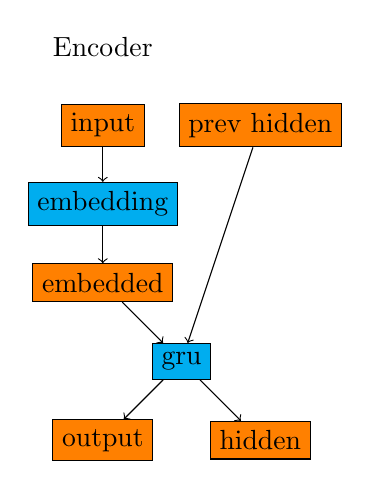
\begin{tikzpicture}

\node at (0, 1) {Encoder};

\node[draw,fill=orange](input) at (0,0) {input};
\node[draw,fill=orange](prev hidden) at (2,0) {prev hidden};

\node[draw,fill=cyan](embedding) at (0,-1) {embedding};

\node[draw,fill=orange](embedded) at (0,-2) {embedded};

\node[draw,fill=cyan](gru) at (1,-3) {gru};

\node[draw,fill=orange](output) at (0,-4) {output};
\node[draw,fill=orange](hidden) at (2,-4) {hidden};

\draw[->,draw=black] (input) to (embedding);
\draw[->,draw=black] (prev hidden) to (gru);

\draw[->,draw=black] (embedding) to (embedded);

\draw[->,draw=black] (embedded) to (gru);

\draw[->,draw=black] (gru) to (output);
\draw[->,draw=black] (gru) to (hidden);

\end{tikzpicture}

\begin{tikzpicture}

\node at (0, 1) {Decoder};

\node[draw,fill=orange](input) at (0,0) {input};
\node[draw,fill=orange](prev hidden) at (2,0) {prev hidden};

\node[draw,fill=cyan](embedding) at (0,-1) {embedding};

\node[draw,fill=lime](relu) at (0,-2) {relu};

\node[draw,fill=cyan](gru) at (1,-3) {gru};

\node[draw,fill=cyan](out) at (0,-4) {out};

\node[draw,fill=lime](softmax) at (0,-5) {softmax};

\node[draw,fill=orange](output) at (0,-6) {output};
\node[draw,fill=orange](hidden) at (2,-6) {hidden};

\draw[->,draw=black] (input) to (embedding);
\draw[->,draw=black] (prev hidden) to (gru);

\draw[->,draw=black] (embedding) to (embedded);

\draw[->,draw=black] (embedded) to (gru);

\draw[->,draw=black] (gru) to (out);
\draw[->,draw=black] (gru) to (hidden);

\draw[->,draw=black] (out) to (softmax);
\draw[->,draw=black] (softmax) to (output);

\end{tikzpicture}


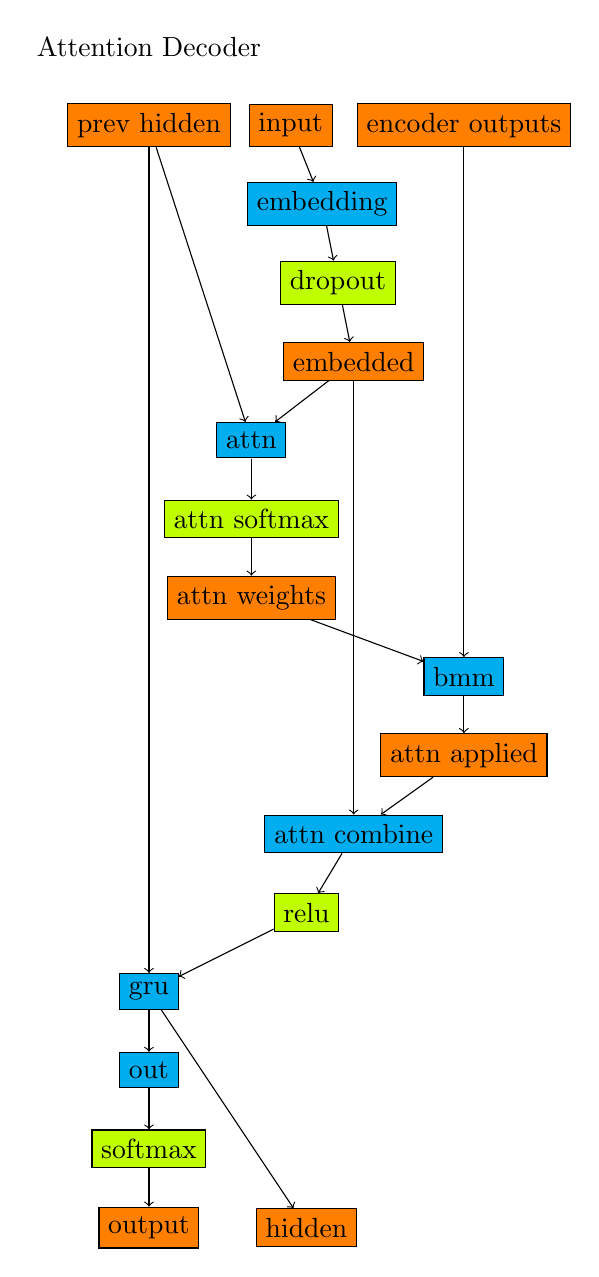
\begin{tikzpicture}

\node at (0, 1) {Attention Decoder};

\node[draw,fill=orange](prev hidden) at (0,0) {prev hidden};
\node[draw,fill=orange](input) at (1.8,0) {input};
\node[draw,fill=orange](encoder outputs) at (4,0) {encoder outputs};

\node[draw,fill=cyan](embedding) at (2.2,-1) {embedding};

\node[draw,fill=lime](dropout) at (2.4,-2) {dropout};

\node[draw,fill=orange](embedded) at (2.6,-3) {embedded};

\node[draw,fill=cyan](attn) at (1.3,-4) {attn};

\node[draw,fill=lime](attn softmax) at (1.3,-5) {attn softmax};

\node[draw,fill=orange](attn weights) at (1.3,-6) {attn weights};

\node[draw,fill=cyan](bmm) at (4,-7) {bmm};

\node[draw,fill=orange](attn applied) at (4,-8) {attn applied};

\node[draw,fill=cyan](attn combine) at (2.6,-9) {attn combine};

\node[draw,fill=lime](relu) at (2,-10) {relu};

\node[draw,fill=cyan](gru) at (0,-11) {gru};

\node[draw,fill=cyan](out) at (0,-12) {out};

\node[draw,fill=lime](softmax) at (0,-13) {softmax};

\node[draw,fill=orange](output) at (0,-14) {output};
\node[draw,fill=orange](hidden) at (2,-14) {hidden};

\draw[->,draw=black] (prev hidden) to (attn);
\draw[->,draw=black] (prev hidden) to (gru);
\draw[->,draw=black] (input) to (embedding);
\draw[->,draw=black] (encoder outputs) to (bmm);

\draw[->,draw=black] (embedding) to (dropout);
\draw[->,draw=black] (dropout) to (embedded);
\draw[->,draw=black] (embedded) to (attn);
\draw[->,draw=black] (embedded) to (attn combine);

\draw[->,draw=black] (attn) to (attn softmax);
\draw[->,draw=black] (attn softmax) to (attn weights);
\draw[->,draw=black] (attn weights) to (bmm);

\draw[->,draw=black] (bmm) to (attn applied);
\draw[->,draw=black] (attn applied) to (attn combine);
\draw[->,draw=black] (attn combine) to (relu);
\draw[->,draw=black] (relu) to (gru);
\draw[->,draw=black] (gru) to (out);
\draw[->,draw=black] (gru) to (hidden);

\draw[->,draw=black] (out) to (softmax);
\draw[->,draw=black] (softmax) to (output);


\end{tikzpicture}


\end{document}